\chapter*{Appendix A: Kriging metamodel}

The Kriging metamodel has already been briefly introduced in chapter \ref{ch:4} but here we want to talk a little bit more on the numerical procedure behind it and also present some implementation example.

The Kriging method was first aimed to make prediction of missing geostatics data (\citet{krige1951statistical}). However this methodology has been further generalized and applied extensively in recent literature as metamodel for large variety of experiments.
The method can treat highly non linear output and can be used to either interpolate or extrapolate response from a sample design set.

In this discussion the $\hat{f}(\boldsymbol{\chi})$ is a model for the function $f(\boldsymbol{\chi})$ and $\hat{y}$ is the model prediction of the true response $y = f(\boldsymbol{\chi})$ that is evaluated at the point $\chi$. $n$ is the number of point in the sample design set and $k$ is the number of input of the experiment.

After the exploration of the design possibilities the database produced is usually organized as $(\mathbf{x_i}, y(\mathbf{x_i}))$  $i=1,...,n$ where
\begin{itemize}
	\item $\mathbf{x_i}$ is the i-th vector element containing the $k$ input parameters for the i-th experiment run
	\item $y_i$ is the scalar response of the experiment for the vector of inputs $\mathbf{x_i}$ \footnote{$y_i$ is always a scalar because even in case of multiple output for an experiment run they are supposed to be uncorrelated. It means that if we had $p$ elements in each $\mathbf{y_i}$ will have to build $p$ metamodels}
\end{itemize}
Also the $n \times k$ matrix containing all the inputs is indicated with $\mathbf{X}$ and the $n \times 1$ vector containing all the responses is indicated as $\mathbf{Y}$

The Kriging response for a new untried input point $\boldsymbol{\chi}$, containing $k$ elements, is given by the linear \textit{predictor}:
\begin{equation}
\hat{y} = \hat{f}(\boldsymbol{\chi}) = \sum_{i=1}^{N} \lambda_i(\mathbf{x}) f(\mathbf{x_i}) =  \sum_{i=1}^{N} \lambda_i(\mathbf{x}) y_i
\end{equation}

$\hat{y}$ is considered to be a new realization of the random Gaussian process that has generated the set of responses $\mathbf{Y}$.
The weights $\lambda_i$ are the solution of a linear system obtained by minimizing the variance of the error between the predictor and the random process.
The best \textit{linear unbiased predictor} BLUP is so obtained finding the weights $\lambda_i$ that minimize:

\begin{equation}
MSE[\hat{y}(\chi)] =  E \left[\left( \hat{f}(\boldsymbol{\chi})  -f(\boldsymbol{\chi}) \right)^2\right] = E \left[\left(\lambda(\chi)\mathbf{Y} -y(\chi)\right)^2\right]
\label{eq:var_err}
\end{equation}

under the unbiasedness condition:

\begin{equation}
E \left[ \hat{f}(\chi)  -f(\chi)\right] =  E \left[ \boldsymbol{\lambda}(\boldsymbol{\chi})\mathbf{Y} -\mathbf{y}(\boldsymbol{\chi})  \right] = 0
\label{eq:unb_cond}
\end{equation}
this relation means that the predictor and the Gaussian process have the same mean value for every new point $\boldsymbol{\chi}$.

The equation \eqref{eq:unb_cond} is further developed yielding:
\begin{equation}
E \left[ \hat{f}(\chi)  -f(\chi)\right] = \boldsymbol{\lambda} E \left[ f(\mathbf{X})  \right] - E \left[ f(\boldsymbol{\chi})  \right] = \sum_{i=1}^{n} \lambda_i(\boldsymbol{\chi}) \mu(\mathbf{x_i}) - \mu(\boldsymbol{\chi}) = 0
\label{eq:unb_cond2}
\end{equation}
where $\mu(\boldsymbol{\chi})$ is the mean value of the true function at the point $\chi$, instead $\mu(\mathbf{x_i})$ is the mean of all the realizations collected for the database.

Different type of Kriging approximation exist accordingly on how $\mu(\boldsymbol{\chi})$ is evaluated:
\begin{itemize}
	\item \textit{simple Kriging} assume that the trend has null value: $\mu(\boldsymbol{\chi}) = 0$
	\item \textit{ordinary Kriging} assume that the trend is an unknown constant: $\mu(\boldsymbol{\chi}) = \mu$
	\item \textit{universal Kriging} assume that the trend is the solution of a generalized \textit{least squares model} in which is possible to decide the order ($n_{\beta}$) \footnote{It means that, for example, taking $n_{\beta}= 2$ the least squared model is quadratic} of the chosen base: $\mu(\boldsymbol{\chi}) = \mathbf{g}(\boldsymbol{\chi})^T \boldsymbol{\beta}$
	Where $\mathbf{g}(\boldsymbol{\chi})$ is the base evaluation at the point $\boldsymbol{\chi}$ and the vector $\boldsymbol{\beta}$ contains the $n_{\beta}$ coefficients of the model.
\end{itemize}

The unbiased condition \eqref{eq:unb_cond2} can be so rewritten, without loss of generality, as:
\begin{eqnarray}
	&& \boldsymbol{ \lambda} (\boldsymbol{\chi}) \mathbf{G}(\mathbf{X}) \boldsymbol{\beta} - \mathbf{g}(\boldsymbol{\chi}) \boldsymbol{\beta} = 0 \nonumber \\
	&& \boldsymbol{\lambda}(\boldsymbol{\chi}) \mathbf{G}(\mathbf{X}) = \mathbf{g}(\boldsymbol{\chi})
\end{eqnarray}
where $\mathbf{G}(\mathbf{X})$ is the $n \times n_{\beta}$ matrix containing the evaluation of the least squared basis functions at all points in $\mathbf{X}$

Also the relation \eqref{eq:var_err} can be manipulated:
\begin{eqnarray}
E \left[\left( \hat{f}(\boldsymbol{\chi})  -f(\boldsymbol{\chi}) \right)^2\right] &=& var(  \hat{f}(\boldsymbol{\chi})  -f(\boldsymbol{\chi}) ) \nonumber \\
&=& var(\hat{f}(\boldsymbol{\chi}))  +var(f(\boldsymbol{\chi})) -2 \; cov( \hat{f}(\boldsymbol{\chi}),f(\boldsymbol{\chi})) \nonumber \\
&=& var( \sum_{i=1}^{n}\lambda_i(\boldsymbol{\chi}) f(\mathbf{x_i}) )  +var(f(\boldsymbol{\chi})) -2 \; cov( \sum_{i=1}^{n}\lambda_i(\boldsymbol{\chi}) f(\mathbf{x_i}),f(\boldsymbol{\chi})) \nonumber \\
&=&  \sum_{i=1}^{n} \sum_{j=1}^{n} \lambda_i(\boldsymbol{\chi})\lambda_j(\boldsymbol{\chi}) cov(f(\mathbf{x_i}),   f(\mathbf{x_j})) +var(f(\boldsymbol{\chi})) -2 \;  \sum_{i=1}^{n}\lambda_i(\boldsymbol{\chi}) cov(f(\mathbf{x_i}),f(\boldsymbol{\chi})) \nonumber \\
&=& \sum_{i=1}^{n} \sum_{j=1}^{n} \lambda_i(\boldsymbol{\chi})\lambda_j(\boldsymbol{\chi}) cov(\mathbf{x_i}, \mathbf{x_j}) +var(f(\boldsymbol{\chi})) -2 \;  \sum_{i=1}^{n}\lambda_i(\boldsymbol{\chi}) cov(\mathbf{x_i},\boldsymbol{\chi})
\label{eq:BLURP}
\end{eqnarray}
where $\mathbf{c} = cov(\mathbf{X},\boldsymbol{\chi})$ is the vector containing the estimated covariance between each point in the input set $\mathbf{X}$ and the point for which we search the estimator $\boldsymbol{\chi}$. Similarly $\mathbf{C}_{ij} =  cov(\mathbf{x_i}, \mathbf{x_j})$ represent the elements in the $n \times n$ matrix containing the correlation estimates for each point in $\mathbf{X}$.

Possible estimation functions for the covariance matrix are listed in the next section \ref{sec:cov}

The derivative of the relation \eqref{eq:BLURP} in respect to $\boldsymbol{ \lambda}$ is posed equal to zero in order to minimize the Kriging error, yielding the final relation:
\begin{equation}
\boldsymbol{\lambda}(\boldsymbol{\chi})^T \mathbf{C} = \mathbf{c}
\end{equation}

Introducing the Lagrangian multiplier $\phi$ for the unbiased constraint is possible to build the the partitioned matrix for the Kriging metamodel:
\begin{equation}
\left(
\begin{array}{c c}
\mathbf{0} & \mathbf{G}^T \\
\mathbf{G} & \mathbf{C}
\end{array}
\right)  \left( 
\begin{array}{c}
\boldsymbol{\phi} \\
\boldsymbol{\lambda}
\end{array}
\right) = \left( 
\begin{array}{c}
\mathbf{g} \\
\mathbf{c}
\end{array}
\right)
\end{equation}

Then by inverting the partitioned matrix the Kriging predictor can be written as:
\begin{equation}
\hat{y}(\boldsymbol{\chi}) = \mathbf{g}(\boldsymbol{\chi})^T \boldsymbol{\beta} + \mathbf{c}(\boldsymbol{\chi})^T \mathbf{R}^{-1} \left( \mathbf{Y} - \mathbf{G}\boldsymbol{\beta} \right)
\end{equation}

The first term $\mathbf{g}(\boldsymbol{\chi})^T \boldsymbol{\beta}$ is usually called \textit{trend function} and the second term is the \textit{Gaussian error model} as a matter of fact $\left( \mathbf{Y} - \mathbf{G}\boldsymbol{\beta} \right)$ is the known vector of differences between the true outputs and the trend function at all the points $\mathbf{X}$ in the database.

We have already said that One of the Kriging metamodel benefits is that the model is exact at the data points. However if it is known that the database present some reliability issue and/or have noise\footnote{common in experimental data}, there is a technique that permits to take into account these effect.
Adding a \textit{nugget} to all entries on the coveriance matrix $\mathbf{C}^* = \mathbf{C} + \eta \mathbf{I}$ the metamodel in no more exact at the data points and also the system condition number is increased.

\subsubsection{Covariance matrix choice}
\label{sec:cov}

In order to give some indication on the choice of the proper covariance function let us first introduce the \textit{semivariogram} concept.
The semivariogram $\gamma$ between two generics points, in the design space of your experiment $\mathbf{x_1}, \mathbf{x_1}$, is defined as:
\begin{eqnarray}
\gamma(\mathbf{x_1}, \mathbf{x_1}) &=& \dfrac{1}{2} E \left[  f(\mathbf{x_1}) -\mu(\mathbf{x_1}) -f(\mathbf{x_1} +\mu(\mathbf{x_2}))^2 \right] \label{eq_semvar1}\\
&=& \dfrac{1}{2} var(f(\mathbf{x_1}) -f(\mathbf{x_1}) ) \nonumber \\
&=& \dfrac{1}{2} var(f(\mathbf{x_1}))  +\dfrac{1}{2} var(f(\mathbf{x_2})) -cov(\mathbf{x_1}, \mathbf{x_2}) \label{eq_semvar2}
\end{eqnarray}

The semivariogram for each datapoint in the database can be directly computed from the \eqref{eq_semvar1} and afterwards the relation \eqref{eq_semvar2} can be used to fit the semivaiogram data with the covariance function.

Lets us clarify the last statements with an example. We chose to replicate the example present in \citet{cavazzuti2012optimization} in which we have an experiment that depend on two variables $x_1$ and $x_2$ and $10$ realization of this experiment. The experiment database is shown in figure \ref{fig:doedata}.

\begin{figure}[t]
	\centering
	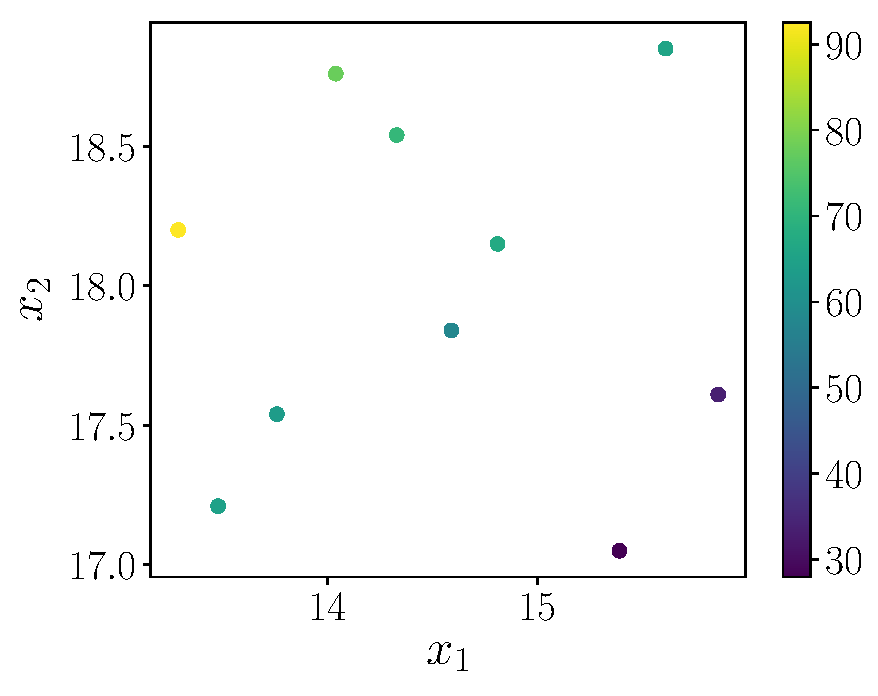
\includegraphics[width=0.5\linewidth]{appendix_a/DOE_data}
	\caption{Experiment data points for the $10$ realizations available. The color map represent the true output realizations of the experiment.}
	\label{fig:doedata}
\end{figure}

The semivariogramm functions, as a function of the eucledian distance between the two points $\mathbf{h}_{ij} = |\mathbf{x}_i - \mathbf{x}_j|$, has been computed using the equation \eqref{eq_semvar1} and is represented in figure \ref{fig:semivariogram} on the left. The same semivariogram has been averaged using a step of distance equal to $0.25$ and the points are shown on the right of figure \ref{fig:semivariogram}.
The correlation function should be be chosen to be the best fit for the averaged semivariogram, so in theory depending on the dataset one could formulate its own covariance model.

\begin{figure}[h]
	\centering
	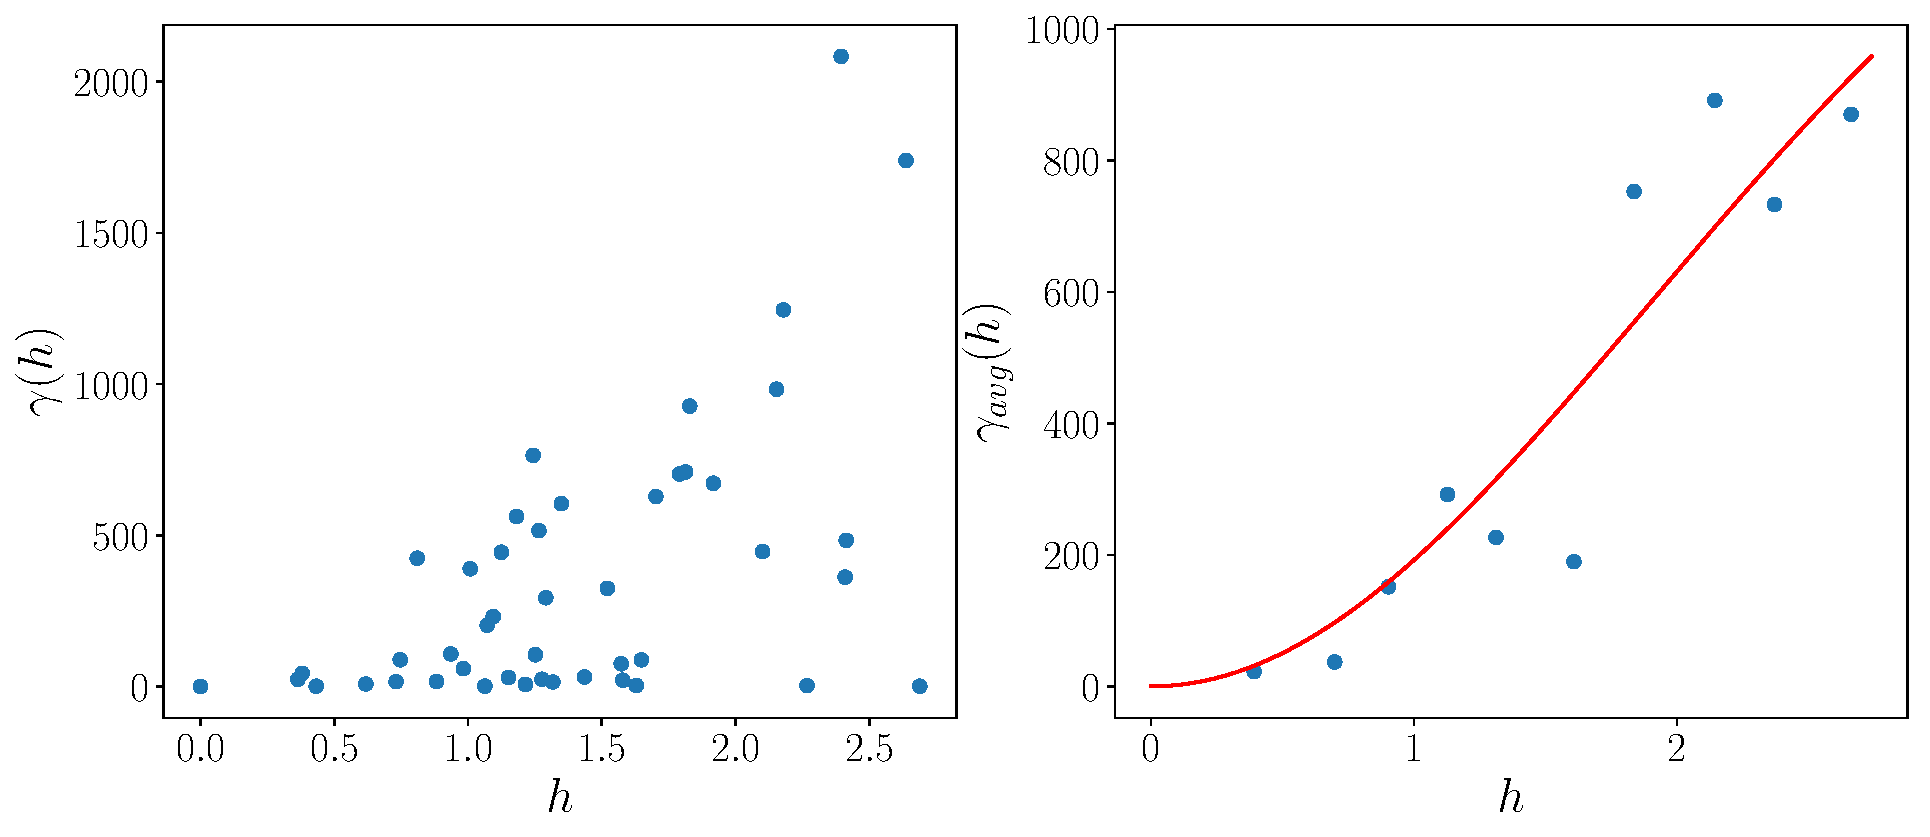
\includegraphics[width=0.9\linewidth]{appendix_a/sem}
	\caption{Left: Semivariogram versus the eucledian distance computed for each data point against all the other.  Right: The blue dots represent the same semivarigram on the left but averaged over a step of distance equal to $0.25$. The red line correspond to the semivariogram computed using the relation \eqref{eq_semvar2} with the covariance model \textit{power exponential} with parameters $\nu=2$, $\theta=1.895$ and $\eta / \sigma=0$.}
	\label{fig:semivariogram}
\end{figure}

What is done in practice is that some parametric families of correlation function has been proposed in literature, for example the \textit{power exponential} correlation function reads:
\begin{equation}
c(\mathbf{x}_{i} , \mathbf{x}_{j})  = \sigma^2 \textrm{exp}\left( -\sum_{j=1}^{k} \theta_k {|\mathbf{x}_{ik} - \mathbf{x}_{jk} |}^\nu \right)
\end{equation}

he kriging metamodel outputs can show different behaviors for different selections of the above three parameters and their setting is thus crucial.
The coefficient $\sigma$ is an amplitude parameter for the correlation function, but it does not entry in the computational model if the nugget $\eta$ is null.
In fact what is generally important is the fraction $\eta / \sigma$ and the exponent $\nu$, larger values of these parameters lead to steeper gradients around the data points. The vector $\bs{\theta}=(\theta_{x_1}, \theta_{x_2})$ is a scaling parameter for the distance $|\mathbf{x_i} - \mathbf{x_j}|$, in this manner the metamodel can include anisotropic effect for each variable of the experiment. If $\boldsymbol{\theta}$ is too small the metamodel surface will be almost equal to the trend function with narrow bumps near the data points. Too large values of $\boldsymbol{\theta}$ will make the surface explode outside the convex hull described by the data points.

This model has been fitted in the previous semivariogram choosing $\nu=2$, $\theta=1.895$ and $\eta / \sigma=0$ and is depicted in the right figure \ref{fig:semivariogram} using a red line. Is possible to see that this model fit well the data points for this experiment.

Another popular model for the covariance function is the \textit{Mat\'ern model}\footnote{the one used in chapter \ref{ch:4}} that reads:
\begin{equation}
c(\mathbf{x}_{i} , \mathbf{x}_{j}) = \sigma^2 \dfrac{2^{1- \nu}}{\Gamma(\nu)} \ \sum_{j=1}^{k} \left( \dfrac{\sqrt{2} \nu |\mathbf{x}_{ik} - \mathbf{x}_{jk} |}{\theta_k} \right)^{\nu} \ \mathcal{K}_{\nu}\left( \dfrac{\sqrt{2} \nu |\mathbf{x}_{ik} - \mathbf{x}_{jk} |}{\theta_k} \right),
\label{eq:matern2}
\end{equation}
where $\mathcal{K}_{\nu}(.)$ is a modified Bessel function and $\Gamma(.)$ is the gamma function.
The parameters that can be used to tune the metamodel are the amplitude parameter $\sigma$, the exponent $\nu$ and the scale vector $\bs{\theta}$ with the same meaning as in the previous correlation function.

To summarize, when choosing the correlation it should be kept in mind:
\begin{itemize}
	\item to well approximate the trend of the averaged semivariogram
	\item that the scale parameter $\boldsymbol{\theta}$ highly change the presence of spurious minima and maxima in the metamodel. The others parameters $\nu$ and $\eta / \sigma$ control the gradient and the exactness of the model around the data points.
\end{itemize}

\subsubsection{Implementation example}

%\begin{minted}[frame=lines, linenos=true]{c++}
%#include <iostream>
%int main() {
%	std::cout << "Hello "
%	<< "world"
%	<< std::endl;
%}
%\end{minted}

\begin{minted}[frame=lines, linenos=true]{python}
	include numpy as np # import the generic verctor library
	include openturns as ot # import the openTurns library
	
	# define the inputs as a n by k array
	x = np.array([[1,0],[2,3 ],[4,6],[-2,0],[9,-3], [3,3],[1,-2],[4,7] ])
	
	# define the outputs as  a n by 1 array
	y = np.array([[10],[2 ],[4],[-2],[9],[3] ,[0], [-1]])
	
	# tranform the array in OT samples
	X = ot.Sample(x)
	Y = ot.Sample(y)
	
	# explicit define the number of input i.e the k number
	dimension = 2  # X.size[1] ??
	
	# distribution = ot.ComposedDistribution([ot.Uniform()]*dimension)
	distribution = ot.ComposedDistribution([ot.Normal()]*dimension)
\end{minted}

\subsubsection{Final observations}

cita tutti i lavori e le librerie da qui hai preso il lavoro.
Metti inoltre il link dal quale hai prodotto i grafici su github